\documentclass[a4paper,11pt,UTF8]{article}
\usepackage{ctex}
\usepackage{amsmath,amsthm,amssymb,amsfonts}
\usepackage{amsmath}
\usepackage[a4paper]{geometry}
\usepackage{graphicx}
\usepackage{microtype}
\usepackage{siunitx}
\usepackage{booktabs}
\usepackage[colorlinks=false, pdfborder={0 0 0}]{hyperref}
\usepackage{cleveref}
\usepackage{esint} 
\usepackage{graphicx}
\usepackage{ragged2e}
\usepackage{pifont}
\usepackage{extarrows}
\usepackage{mathptmx}
\usepackage{float}
\usepackage{caption}
\captionsetup[figure]{name={Figure}}

\title{Microelectronics Circuit Analysis and Design Homework(8th)}
\author{Yuejin Xie \quad U202210333}
\date{Oct 10th, 2023}
\begin{document}
\maketitle
\noindent
5.24 (a) For the circuit in Figure P5.24, determine $V_B$ and $I_E$ such that $V_B = V_C$ .
Assume $\beta = 90$. (b) What value of $V_B$ results in $V_{CE} = 2 $V?
\begin{figure}[H] 
	\centering 
	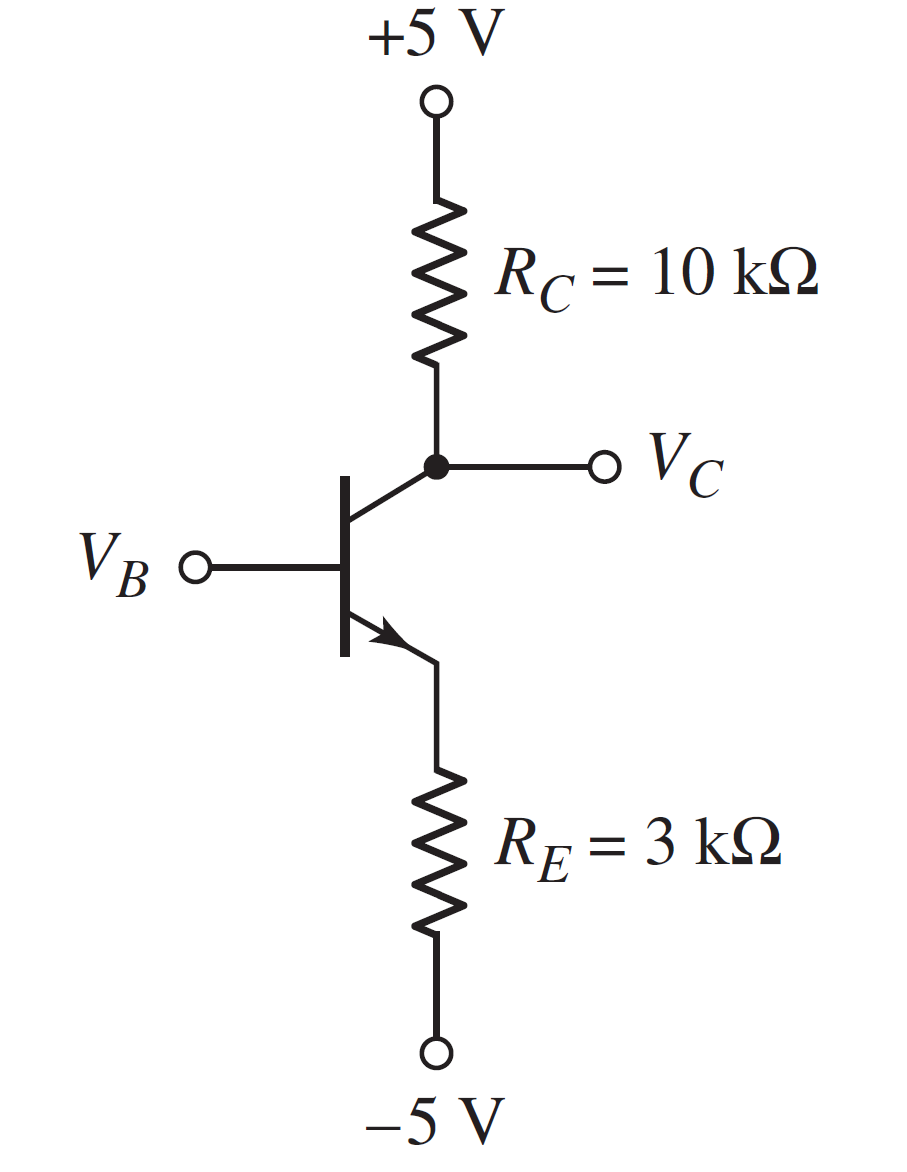
\includegraphics[scale=0.15]{MD5.24.png}
	\caption{Problem 5.24}
\end{figure}
\noindent Solution:\\
(a)Assume the BJT works in the forward-active region:\\
$$\begin{cases}
	\displaystyle I_C=\frac{5-V_C}{R_C}\\
	\displaystyle I_E=\frac{V_{B}-V_{BE(on)-(-5)}}{R_E}\\
	\displaystyle I_E=\frac{1+\beta}{\beta}I_C\\
	V_B=V_C
\end{cases}\Rightarrow
\begin{cases}
	V_B=-2.14\mathrm{V}\\
	I_E=0.72\mathrm{mA}
\end{cases} 
$$
(b)Obviously, the BJT work in the active region, so we have equation:
$$\begin{cases}
	V_C-V_B+V_{BE(on)}=V_{CE}\\
	\displaystyle I_C=\frac{5-V_C}{R_C}\\
	\displaystyle I_E=\frac{V_{B}-V_{BE(on)-(-5)}}{R_E}\\
	\displaystyle I_E=\frac{1+\beta}{\beta}I_C
\end{cases}\Rightarrow 
\begin{cases}
	V_B=-2.44\mathrm{V}\\
	I_E=0.62\mathrm{mA}
\end{cases}
$$
5.43 The common-emitter current gain of the transistor in Figure P5.43 is $\beta = 80$.
Plot the voltage transfer characteristics over the range $0 \leq V_I \leq 5 $V.
\begin{figure}[H] 
	\centering 
	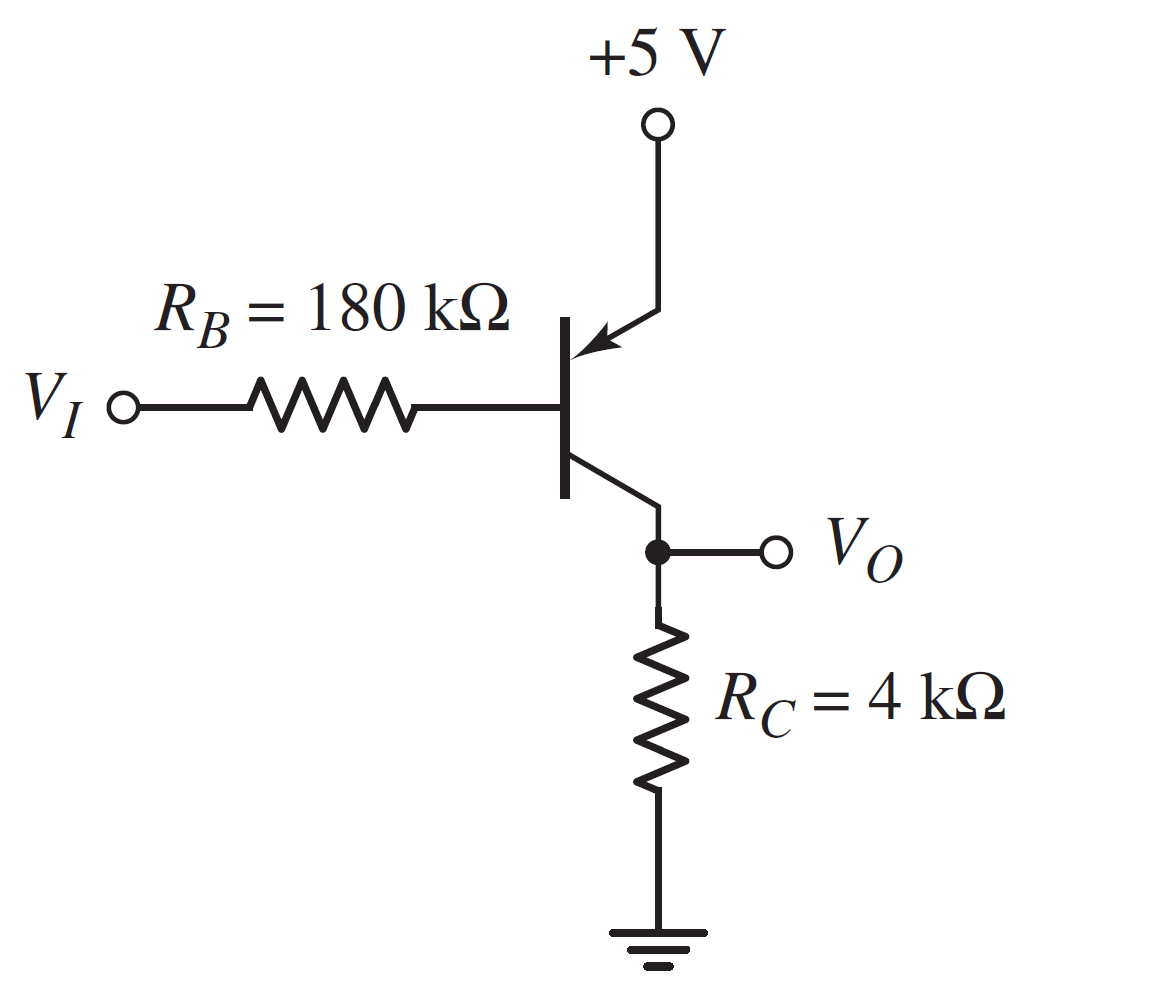
\includegraphics[scale=0.15]{MD5.43.png}
	\caption{Problem 5.43}
\end{figure}
\noindent Solution:\\
It's a PNP BJT\\
case 1: $V_I\in(4.3,5), V_{EB}<0.7$V, the B-E junction isn't conducted, $I_E=0, V_O=0$\\
case 2: When BJT works in saturation region(at sat-point), $V_{EC}=0.2$V, $V_O=4.8$V, $\displaystyle V_I=5-V_{EC(ON)}-\frac{V_O}{\beta R_C}R_B=1.6$V, so when $V_I<1.6$V, $V_O=4.8$V\\
case 3: $V_I\in[1.6,4.3]$, the BJT works in the active region:$$\displaystyle\frac{V_O}{R_C}=\beta\frac{5-V_{BE(ON)}-V_I}{R_B}\Rightarrow V_O=-\frac{16}{9}V_I+\frac{344}{45}$$\\
5.70 For the circuit in Figure P5.70, let $R_C = 2.2 \mathrm{k\Omega}$, $R_E = 2 \mathrm{k\Omega}$, $R_1 = 10 \mathrm{k\Omega}$,
$R_2 = 20 \mathrm{k\Omega}$, and $\beta = 60$. (a) Find $R_{T H}$ and $V_{T H}$ for the base circuit.
(b) Determine $I_{BQ}$, $I_{CQ}$, $V_E$ , and $V_C$.
\begin{figure}[H] 
	\centering 
	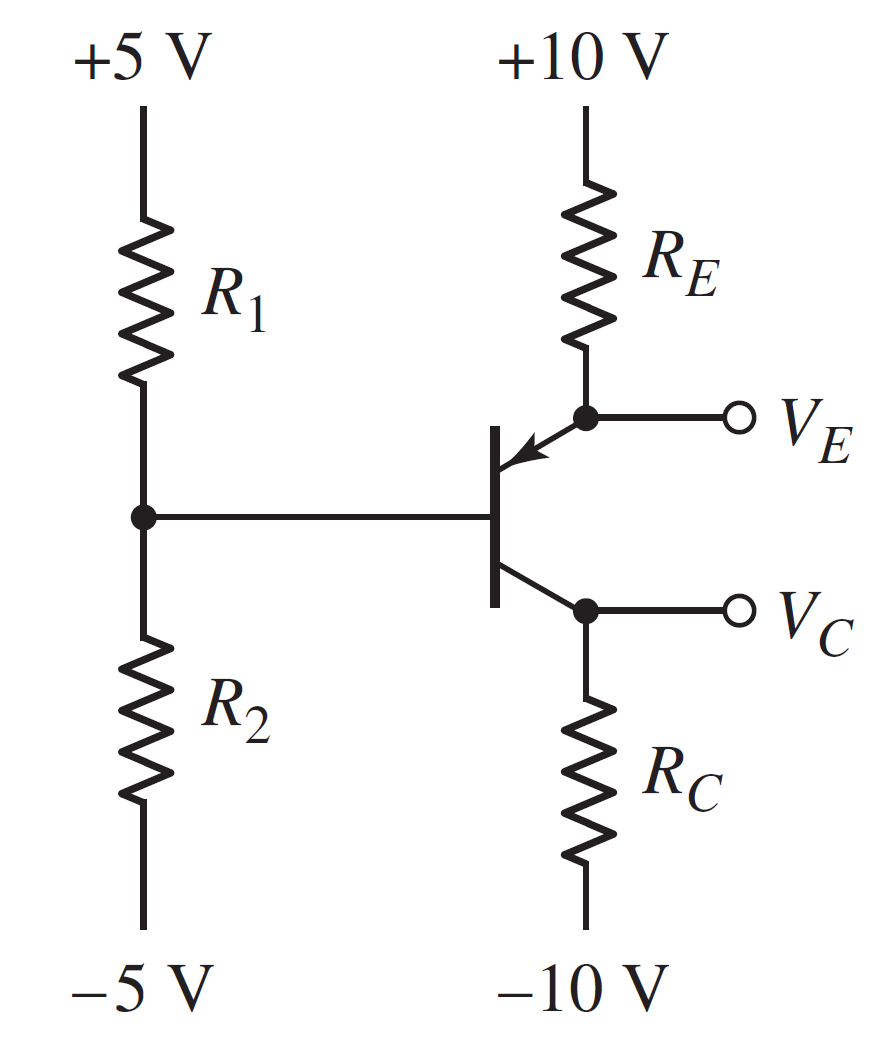
\includegraphics[scale=0.15]{MD5.70.png}
	\caption{Problem 5.70}
\end{figure}
6.8 The parameters of each transistor in the circuits shown in Figure P6.8 are
$\beta = 130$, $V_A = 80 $V, and $I_{CQ} = 0.2 $mA. Determine the output resistance
$R_o$ for each circuit.
\begin{figure}[H] 
	\centering 
	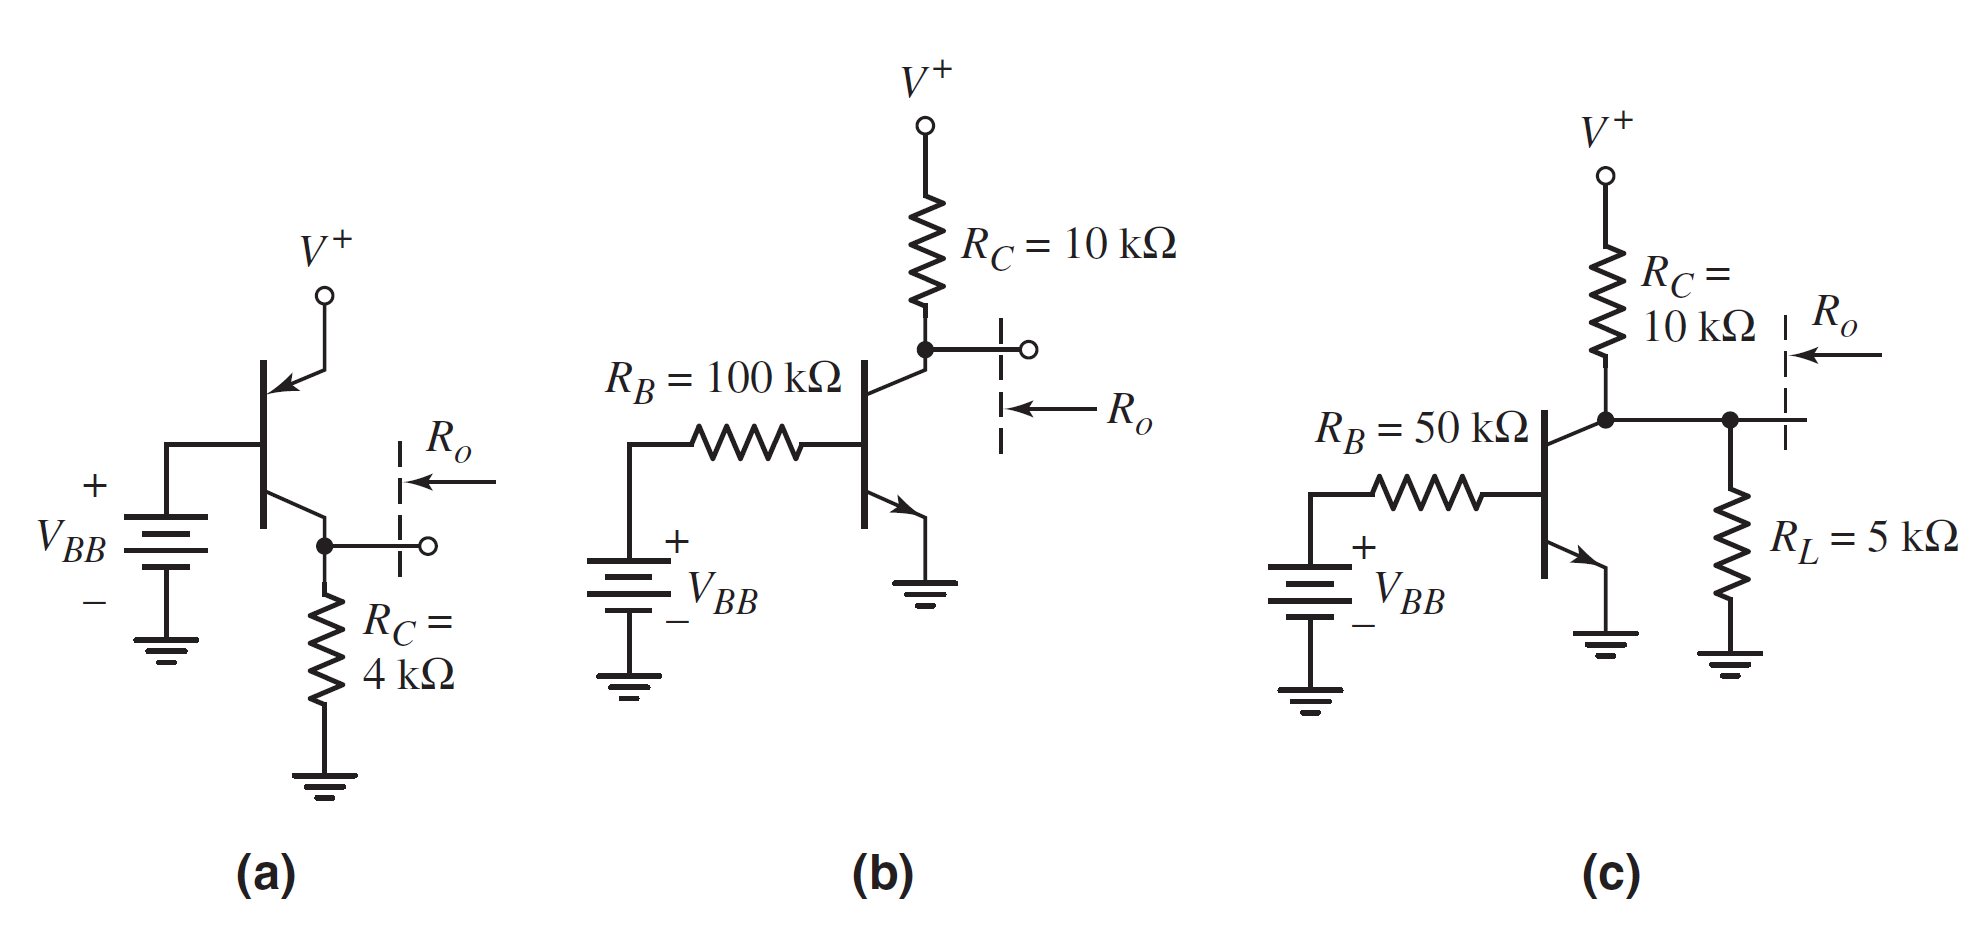
\includegraphics[scale=0.3]{MD6.8.png}
	\caption{Problem 6.8}
\end{figure}
6.18 The signal source in Figure P6.18 is $v_s = 5 \sin\omega t $mV. The transistor parameters
are $\beta = 120$ and $V_A =\infty$. (a) (i) Design the circuit such that
$I_{CQ} = 0.25 $mA and $V_{CEQ} = 3 $V. (ii) Find the small-signal voltage gain
$A_v = v_o/v_s$ . (iii) Find $v_o(t)$. (b) Repeat part (a) for $R_S = 0$.
\begin{figure}[H] 
	\centering 
	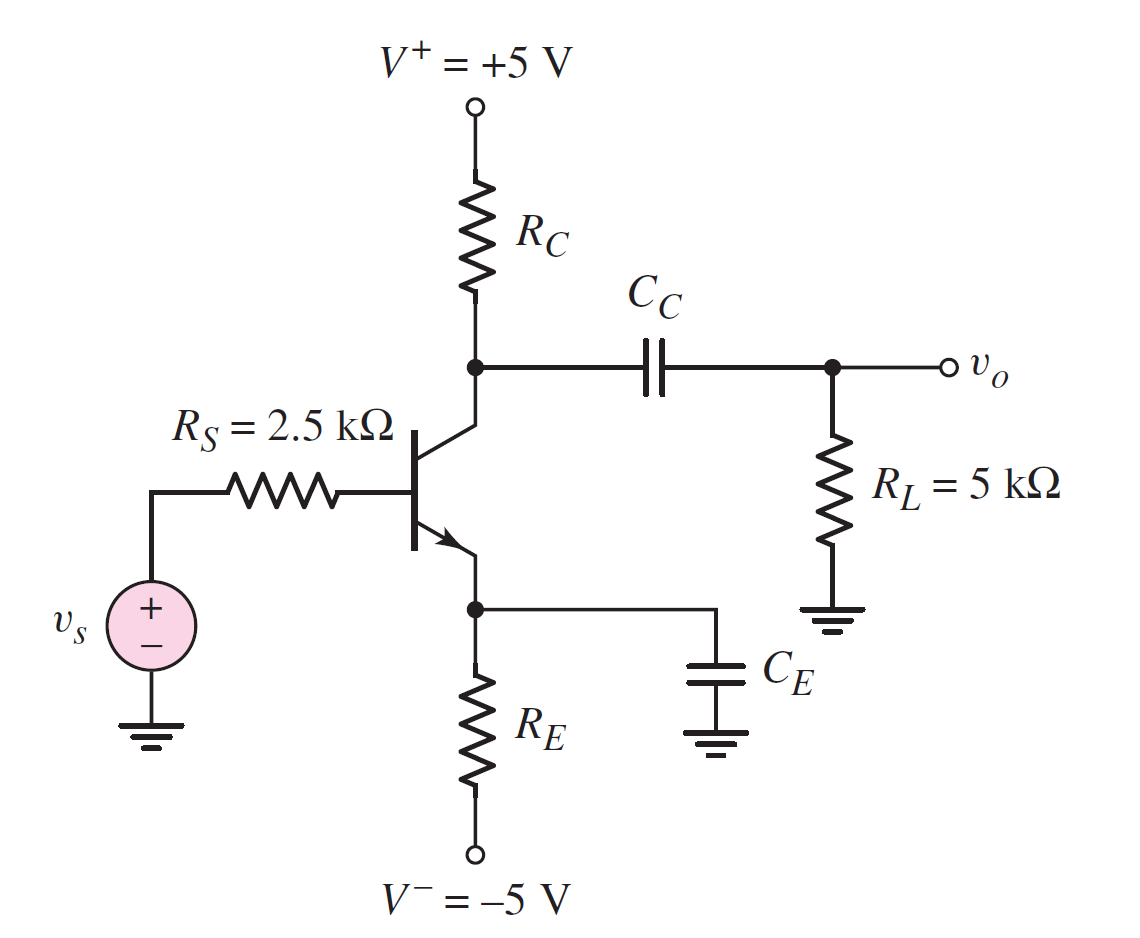
\includegraphics[scale=0.3]{MD6.18.png}
	\caption{Problem 6.18}
\end{figure}
6.33 For the circuit in Figure P6.15, let $\beta = 100$, $V_A =\infty$, $R_E = 12.9 \mathrm{k\Omega}$, and
$R_C = 6 \mathrm{k\Omega}$. Determine the maximum undistorted swing in the output
voltage if the total instantaneous C–E voltage is to remain in the range
$1 \leq v_{CE} \leq 9 $V and if the total instantaneous collector current is to remain
greater or equal to $50 \mu$ A.
\begin{figure}[H] 
	\centering 
	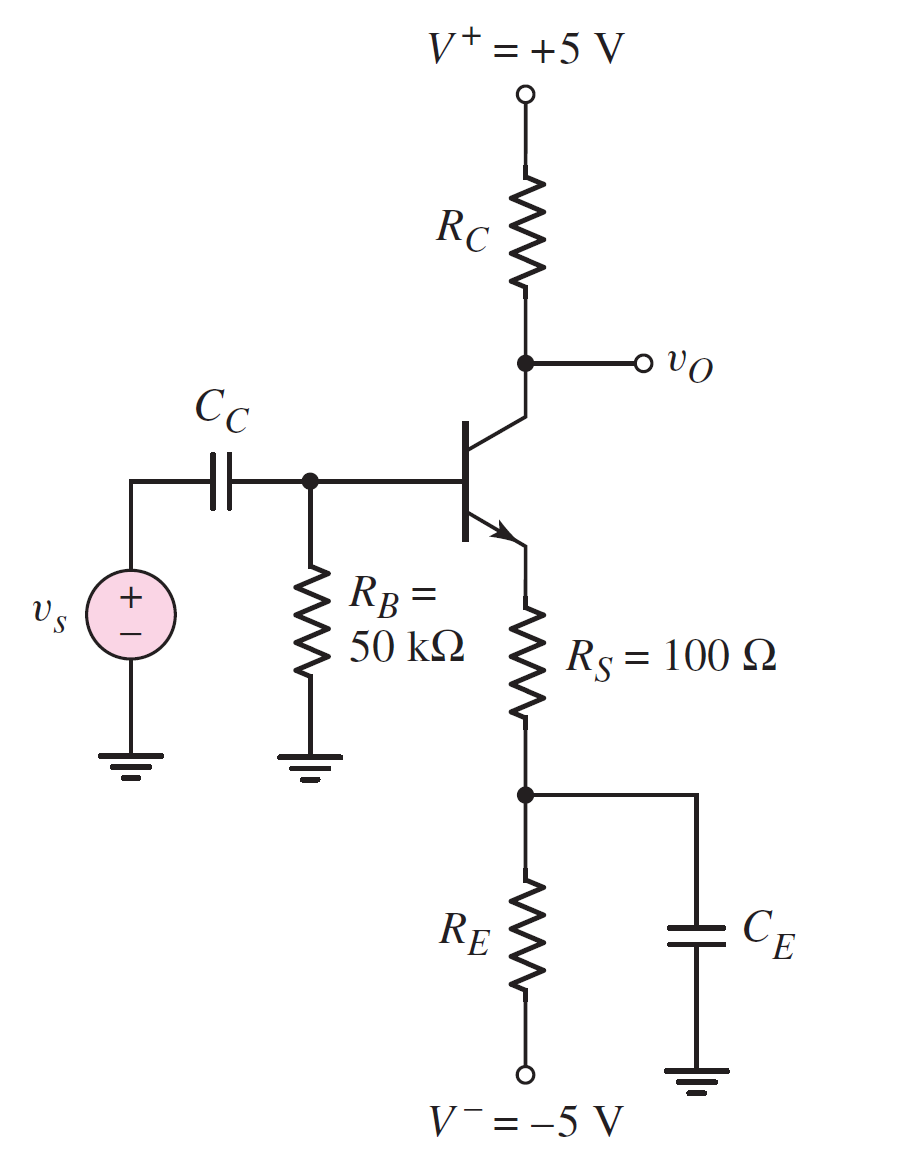
\includegraphics[scale=0.3]{MD6.33.png}
	\caption{Problem 6.33}
\end{figure}
6.39 For the circuit in Figure P6.24, the transistor parameters are $\beta = 100$ and
$V_A =\infty$. (a) Determine the maximum undistorted swing in the output
voltage if the total instantaneous E–C voltage is to remain in the range
$1 \leq v_{EC} \leq 9 $V. (b) Using the results of part (a), determine the range of collector
current.
\begin{figure}[H] 
	\centering 
	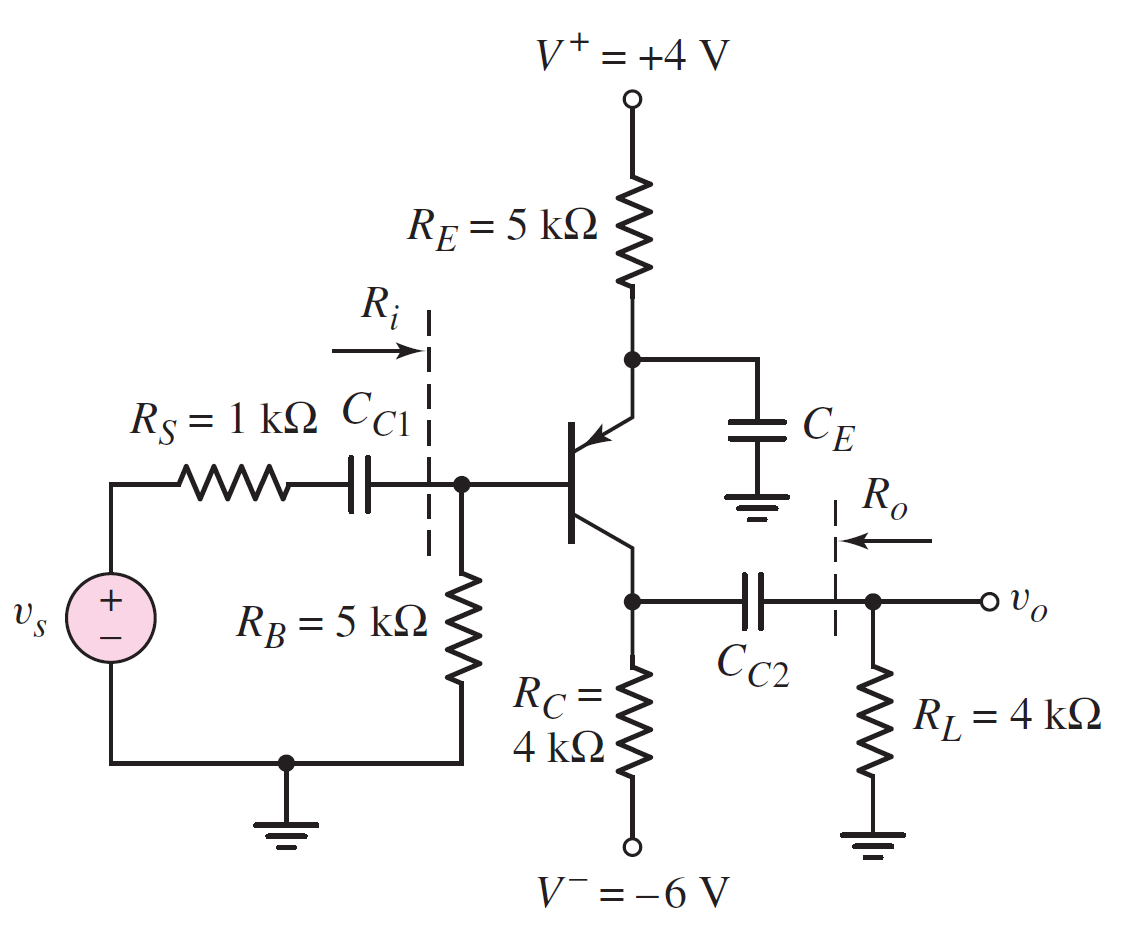
\includegraphics[scale=0.3]{MD6.39.png}
	\caption{Problem 6.39}
\end{figure}
6.65 Consider the circuit shown in Figure P6.69. The transistor has parameters
$\beta = 60$ and $V_A =\infty$. (a) Determine the quiescent values of $I_{CQ}$ and $V_{CEQ}$.
(b) Determine the small-signal voltage gain $A_v = v_o/v_s$.
\begin{figure}[H] 
	\centering 
	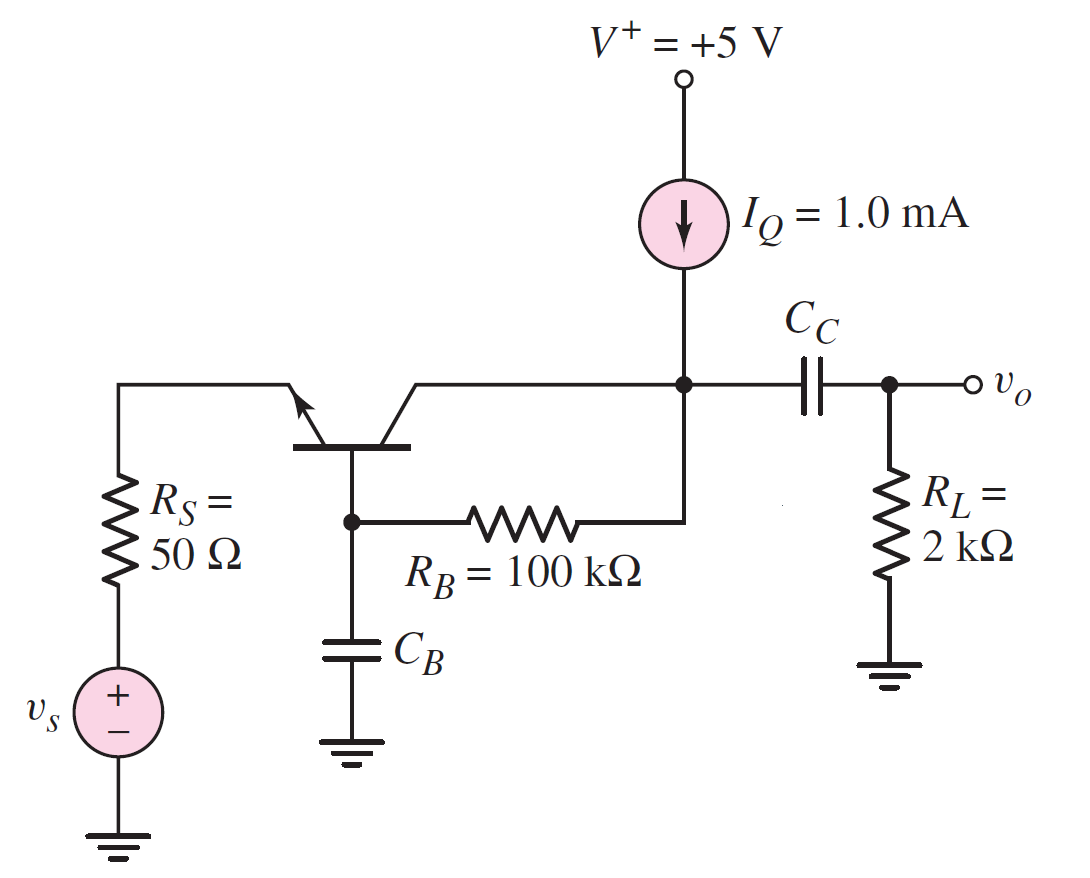
\includegraphics[scale=0.3]{MD6.69.png}
	\caption{Problem 6.69}
\end{figure}
\end{document}